\begin{frame}
  \frametitle{\problemtitle}
  \begin{block}{Problem}
    You are given a region consisting of some cells in a rectangular grid.
    Find the longest possible length such that the region can be divided into squares of that side length.
  \end{block}
  \begin{center}
    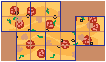
\includegraphics[width=0.6\textwidth]{pizza.pdf}
  \end{center}
\end{frame}
\begin{frame}
  \frametitle{\problemtitle}
  \begin{block}{Solution}
    \begin{itemize}
      \item Testing whether a given length is possible can be done in $\mathcal{O}(h\cdot w)$:

        \begin{itemize}
          \item Scan over the grid from top left to bottom right
          \item Whenever an unmarked cell is encountered, it must be the top left corner of a square
          \item Check if a square can be placed here and mark all cells belonging to it, then continue scanning
          \item In the end, check if all cells of the region have been marked
          \item The time does not depend on the size of the square!
        \end{itemize}
      \item Testing all side lengths from $1$ to $\min(h, w)$ is too slow for the given bounds
      \item \emph{Key Improvement}: Only test side lengths $k$ such that $k^2$ divides $n$, the number of cells
        \begin{itemize}
          \item The worst case in the given bounds is $n = 2\,822\,400 = 2^8 \cdot 3^2 \cdot 5^2 \cdot 7^2$, which has $40$ square divisors
        \end{itemize}
      \item With this improvement, the solution is fast enough
    \end{itemize}
  \end{block}
\end{frame}
